\documentclass[../main.tex]{subfiles}
\begin{document}

\chapter{Basic Concepts of Numerical Analysis with Taylor's Theorem } 
\addcontentsline{toc}{section}{Chapter 2:Basic Concepts of Numerical 
Analysis with Taylor's Theorem }

\section{WHAT IS NUMERICAL ANALYSIS?}

Outside the realm of pure mathematics, most practicing scientists and engineers are 
not concerned with finding exact answers to problems. Indeed, living in a finite 
universe, we have no way of exactly measuring physical quantities and even if we 
did, the exact answer would not be of much use. Just a single irrational number, 
such as\\


$\pi = 3.1415926535897932384626433832795028841971693993751058209749...$,\\ 


where the digits keep going on forever without repetition or any known pattern, 
has more information in its digits than all the computers in the world could 
possibly ever store. To help motivate some terminology, we bring forth a couple 
of examples. \\

Suppose that Los Angeles County is interested in finding out the amount of water 
contained in one of its reserve drinking water reservoirs. It hires a contracting firm 
to measure this amount. The firm begins with a large-scale pumping device to take 
care of most of the water, leaving only a few gallons. After this, they bring out a 
more precise device to measure the remainder and come out with a volume of 
12,564,832.42 gallons. To get a second opinion, the county hires a more 
sophisticated engineering firm (that charges 10 times as much) and that uses more 
advanced measuring devices. Suppose this latter firm came up with the figure 
12,564,832.3182. Was the first estimate incorrect? Maybe not, perhaps some 
evaporation or spilling took place—so there cannot really be an exact answer to 
this problem. Was it really worth the extra cost to get this more accurate estimate? 
Most likely not—even an estimate to the nearest gallon would have served equally 
well for just about any practical purposes.\\

Suppose next that the Boeing Corporation, in the design and construction of a 
new 767 model jumbo jet, needs some wing rivets. The engineers have determined 
the rivets should have a diameter of 2.75 mm with a tolerance (for error) of 
.000025 mm. Boeing owns a precise machine that will cut such rivets to be of 
diameter 2.75±.000006mm. But they can purchase a much more expensive 
machine that will produce rivets of diameters 2.75±.0000001 mm (60 times as 
accurate). Is it worth it for Boeing to purchase and use this more expensive 
machine? The aeronautical engineers have determined that such an improvement 
in rivets would not result in any significant difference in the safety and reliability 
of the wing and plane; however, if the error exceeds the given tolerance, the wings 
may become unstable and a safety hazard.\\

In mathematics, there are many problems and equations (algebraic, differential, 
and partial differential) whose exact solutions are known to exist but are difficult, 
very time consuming, or impossible to solve exactly. But for many practical 
purposes, as evidenced by the previous examples, an estimate to the exact answer 
will do just fine, provided that we have a guarantee that the error is not too large. 
So, here is the basic problem in numerical analysis:

We are interested in a solution x (= \textbf{exact answer}) to a problem or equation.
We would like to find an estimate x*(=\textbf{ approximation}) so that |x-x*|(= \textbf{the actual error}) is no more than the 
maximum \textbf{tolerance} (= $\epsilon$), i.e.,$ |x-x*| < \epsilon$ . The maximum tolerated error will be 
specified ahead of time and will depend on the particular problem at hand. What 
makes this approximation problem very often extremely difficult is that we usually 
do not know x and thus, even after we get x*, we will have no way of knowing 
the actual error. But regardless of this, we still need to be able to guarantee that it 
is less than $\epsilon$. Often more useful than the actual error is the relative error, which 
measures the error as a ratio in terms of the magnitude of the actual quantity; i.e., it 
is defined by\\

relative error $=\frac{|x-x*|}{|x|}$\\

provided, of course, that $x \neq 0$.\\

\textbf {EXAMPLE 2.1:} In the Los Angeles reservoir measurement problem given earlier, suppose we took the exact answer to be the engineering firm's estimate, $x=$ $12,564,832.3182$ gallons, and the contractor's estimate as the approximation $x^{*}=$ $12,564,832.42$. Then the error of this approximation is $\left|x-x*\right|=0.1018$ gallons,\\

\textbf {EXAMPLE 2.2:} In the Boeing Corporation's rivet problem above, the maximum tolerated error is $.000025 mm$, which translates to a maximum relative error of (divide by $x=2.75$ ) $0.000009$. The machine they currently have would yield a maximum relative error of $0.000006 / 2.75=0.000002$ and the more expensive machine they were considering would guarantee a maximum relative error of no more than $0.0000001 / 2.75=3.6364 \times 10^{-8}$.

For the following reasons, we have chosen Taylor's theorem as a means to launch 
the reader into the realm of numerical analysis. First, Taylor's theorem is at the 
foundation of most numerical methods for differential equations, the subject of this 
book. Second, it covers one of those rare situations in numerical analysis where 
quality error estimates are readily available and thus errors can be controlled and 
estimated quite effectively. Finally, most readers should have some familiarity 
with Taylor's theorem from their calculus courses.\\

Most mathematical functions are very difficult to compute by just using the basic 
mathematical operations: +, -, x, * . How, for example, would we compute
$cos(27^{\circ})$ just using these operations? One type of function that is possible to 
compute in this way is a polynomial. A polynomial in the variable x is a function 
of the form: 

$$
p(x)=a_{n} x^{n}+\cdots+a_{2} x^{2}+a_{1} x+a_{0},
$$
where $a_{n}, \cdots a_{2}, a_{1}, a_{0}$ are any real numbers. If $a_{n} \neq 0$, then we say that the degree of $p(x)$ equals $n$. Taylor's theorem from calculus shows how to use polynomials to approximate a great many mathematical functions to any degree of accuracy. In Section 2.2, we will introduce the special kind of polynomial (called Taylor polynomials) that gets used in this theorem and in Section $2.3$ we discuss the theorem and its uses.\\
ś
\hrule width \hsize \kern 1pt \hrule width \hsize height 0.4pt

\hspace{0.1cm}

\textbf{EXERCISES 2.1: }

\begin{enumerate}

\item If $x=2$ is approximated by $x^{*}=1.96$, find the actual error and the relative error.
\item If $\pi(=x)$ is approximated by $x^{*}=3 \frac{1}{8}$ (as was done by the ancient Babylonians, c. $2000 \mathrm{BC}$ ), find the actual error and the relative error.
\item If $x=10000$ is approximated by $x^{*}=9999.96$, find the actual error and the relative error.
\item If $x=5280$ feet (one mile) is approximated by $x^{\circ}=5281$ feet, find the actual and relative errors.
\item If $x=0.76$ inches and the relative error of an approximation is known to be $0.05$, find the possible values for $x^{*}$.
\item If $x=186.4$ and the relative error of an approximation is known to be $0.001$, find the possible values for $x^{*}$.
\item A civil engineering firm wishes to order thick steel cables for the construction of a span bridge. The cables need to measure 2640 feet in length with a maximum tolerated relative error of $0.005$. Translate this relative error into an actual tolerated maximum discrepancy from the ideal 2640 foot length.

\end{enumerate}

\section{TAYLOR POLYNOMIALS} \label{subsection}

Suppose that we have a mathematical function $f(x)$ that we wish to approximate near $x=a$. \textbf{The Taylor polynomial of order} $n, p_{n}(x)$, for this function \textbf{centered at (or about)} $x=a$ is that polynomial of degree of at most $n$ that has the same values as $f(x)$ and its first $n$ derivatives at $x=a$. The definition requires that $f(x)$ possess $n$ derivatives at $x=a$. Since derivatives measure rates of change of functions, the Taylor polynomials are designed to mimic the behavior of the function near $x=a$. The following example will demonstrate this property.\\

\textbf {EXAMPLE 2.3:} Find formulas for, and interpret, the order-zero and order-one Taylor polynomials $p_{0}(x)$ and $p_{1}(x)$ of a function $f(x)$ (differentiable) at $x=a$.\\

SOLUTION: The zero-order polynomial $p_{0}(x)$ has degree at most zero, and so must be a constant function. But by its definition, we must have $p_{0}(a)=f(a)$. Since $p_{0}(x)$ is constant this means that $p_{0}(x)=f(a)$ (a horizontal line function). The first-order polynomial $p_{1}(x)$ must satisfy two conditions:


\begin{equation}\label{eq:1} \tag{1}
p_{1}(a)=f(a) \text { and } p_{1}^{\prime}(a)=f^{\prime}(a)
\end{equation}


\begin{figure}[H]
\centering
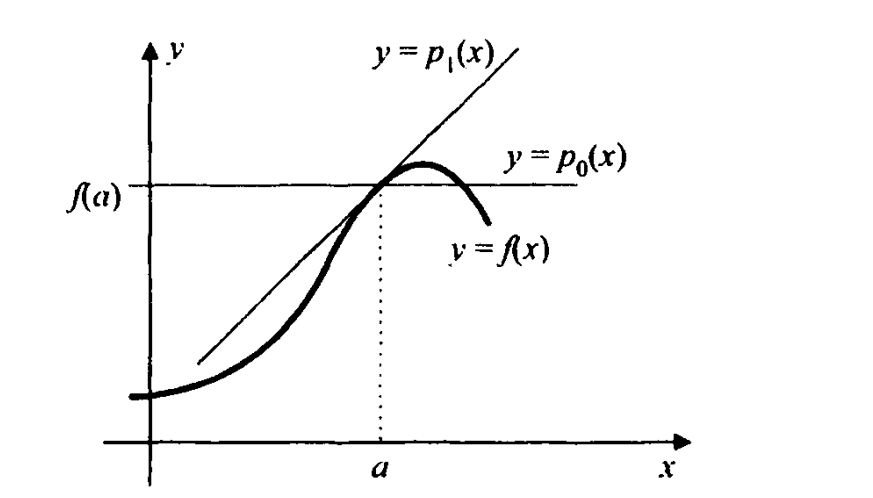
\includegraphics[width=0.8\textwidth,height=65mm]{fig21}
\caption{ Illustration of a graph of a function $y=f(x)$ (heavy black curve) together with its zero-order Taylor polynomial $p_{0}(x)$ (horizontal line) and first-order Taylor polynomial $p_{1}(x)$ (slanted tangent line). }
\label{fig:fig_2_1}
\end{figure}

Since $p_{1}(x)$ has degree at most one, we can write $p_{1}(x)=m x+b$, i.e., $p_{1}(x)$ is just a line with slope $m$ and $y$-intercept $b$. If we differentiate this equation and use the second equation in (1), we get that $m=f^{\prime}(a)$. We now substitute this in for $m$, put $x=a$ and use the first equation in (1) to find that $f(a)=p_{1}(a)$ $=f^{\prime}(a) a+b$. Solving for $b$ gives $b=f(a)-f^{\prime}(a) a$. So putting this all together yields that $p_{1}(x)=m x+b=f^{\prime}(a) x+f(a)-f^{\prime}(a) a=f(a)+f^{\prime}(a)(x-a)$. This is just the tangent line to the graph of $y=f(x)$ at $x=a$. These two polynomials are illustrated in Figure 2.1.

In general, it can be shown that the Taylor polynomial of order $n$ is given by the following formula:

\begin{equation}\label{eq:2} \tag{2}
\begin{array}{r}
p_{n}(x)=f(a)+f^{\prime}(a)(x-a)+\frac{1}{2} f^{\prime \prime}(a)(x-a)^{2}+\frac{1}{3 !} f^{\prime \prime \prime}(a)(x-a)^{3}+ \\
\cdots+\frac{1}{n !} f^{(n)}(a)(x-a)^{n},
\end{array}
\end{equation}

where we recall that the factorial of a positive integer $k$ is given by:
$$
k !=\left\{\begin{array}{l}
1, \text { if } k=0 \\
1 \cdot 2 \cdot 3 \cdots(k-1) \cdot k, \text { if } k=1,2,3, \cdots .
\end{array}\right.
$$
Since $0 !=1 !=1$, we can use Sigma-notation to rewrite this more simply as:

\begin{equation}\label{eq:3} \tag{3}
p_{n}(x)=\sum_{k=0}^{n} \frac{1}{k !} f^{(k)}(a)(x-a)^{k} .
\end{equation}
We turn now to some specific examples:\\

\textbf{EXAMPLE 2.4: }

 (a) For the function $f(x)=\cos (x)$, compute the following Taylor polynomials at $x=0: p_{1}(x), p_{2}(x), p_{3}(x)$, and $p_{8}(x)$.

(b) Use MATLAB to find how each of these approximates $\cos \left(27^{\circ}\right)$ and then find the actual error of each of these approximations.

(c) Find a general formula for $p_{n}(x)$.

(d) Using an appropriate MATLAB graph, estimate the length of the largest interval $[-a, a]=\{|x| \leq a\}$ about $x=0$ that $p_{8}(x)$ can be used to approximate $f(x)$ with an error always less than or equal to $0.2$. What if we want the error to be less than or equal to $0.001$ ? \\

SOLUTION: Part (a): We see from formula (2) or (3) that each Taylor polynomial is part of any higher-order Taylor polynomial. Since $a=0$ in this example, formula (2) reduces to:

\begin{equation}\label{eq:4} \tag{4}
\begin{aligned}
p_{n}(x)=f(0)+f^{\prime}(0) x+& \frac{1}{2} f^{\prime \prime}(0) x^{2}+\frac{1}{3 !} f^{\prime \prime \prime}(0) x^{3}+\cdots \\
&+\frac{1}{n !} f^{(n)}(0) x^{n}=\sum_{k=0}^{n} \frac{1}{k !} f^{(k)}(0) x^{k} .
\end{aligned}
\end{equation}

A systematic way to calculate these polynomials is by constructing a table for the derivatives:

\begin{center}
\begin{tabular}{|c|c|c|}
\hline
$\mathbf{n}$ & $f^{(n)}(x)$ & $f^{(n)}(0)$ \\
\hline
$\mathbf{0}$ & $\cos (x)$ & 1 \\
\hline
$\mathbf{1}$ & $-\sin (x)$ & 0 \\
\hline
2 & $-\cos (x)$ & $-1$ \\
\hline
$\mathbf{3}$ & $\sin (x)$ & 0 \\
\hline
$\mathbf{4}$ & $\cos (x)$ & 1 \\
\hline
$\mathbf{5}$ & $-\sin (x)$ & 0 \\
\hline
\end{tabular}
\end{center}
We could continue on, but if one notices the repetitive pattern (when $n=4$, the derivatives go back to where they began), this can save some time and help with finding a formula for the general Taylor polynomial $p_{n}(x)$. Using formula (4) in conjunction with the table (and indicated repetition pattern), we conclude that:

$$
p_{1}(x)=1, p_{2}(x)=1-\frac{x^{2}}{2}=p_{3}(x) \text {, and } p_{8}(x)=1-\frac{x^{2}}{2}+\frac{x^{4}}{4 !}-\frac{x^{6}}{6 !}+\frac{x^{8}}{8 !} \text {. }
$$

Part (b): To use these polynomials to approximate $\cos \left(27^{\circ}\right)$, we of course need to take $x$ to be in radians, i.e., $x=27^{\circ}\left(\frac{\pi}{180^{\circ}}\right)=.4712389 \ldots .$ Since two of these Taylor polynomials coincide, there are three different approximations at hand for $\cos \left(27^{\circ}\right)$. In order to use MATLAB to make the desired calculations, we introduce a relevant MATLAB function:

\begin{figure}[H]
\centering
\begin{boxedverbatim}
To compute n! in MATLAB, use either: $ factorial (n), or gamma (n+1)$
\end{boxedverbatim}
\end{figure}


\begin{verbatim}
>>x=27*pi/180;
>>format long
>>p1=1; p2=1-x^2/2
	-> 0.88896695048774
>> p8=p2+x^4/gamma(5)-x^6/gamma(7)+x^8/gamma(9)
-> 0.89100652433693
>> abs(p1-cos(x)) %abs, as you guessed, stands for absolute value
->0.10899347581163
>>abs(p2-cos(x)) -»0.00203957370062
>>abs (p8-cos (x) ) -» 1.485654932409375e-010 
\end{verbatim}

Thus for example, to get $5 !=120$, we could either type $\gg>$ factorial $(5)$ or >gamma (6). Now we calculate:

Transcribing these into usual mathematics notation, we have the approximations for $\cos \left(27^{\circ}\right)$ :
$$
p_{1}\left(27^{\circ}\right)=1, p_{2}\left(27^{\circ}\right)=p_{3}\left(27^{\circ}\right)=.888967 \ldots, p_{8}\left(27^{\circ}\right)=.89100694 \ldots,
$$
which have the corresponding errors:
$$
\begin{aligned}
&\left|p_{1}\left(27^{\circ}\right)-\cos \left(27^{\circ}\right)\right|=0.1089 \ldots, \\
&\left|p_{2}\left(27^{\circ}\right)-\cos \left(27^{\circ}\right)\right|=\left|p_{3}\left(27^{\circ}\right)-\cos \left(27^{\circ}\right)\right|=0.002039 \ldots, \text { and } \\
&\left|p_{8}\left(27^{\circ}\right)-\cos \left(27^{\circ}\right)\right|=1.4856 \times 10^{-10} .
\end{aligned}
$$
This demonstrates quite clearly how nicely these Taylor polynomials serve as approximating tools. As expected, the higher degree Taylor polynomials do a better job approximating but take more work to compute.\\

Part (c): Finding the general formula for the $n$ th-order Taylor polynomial $p_{n}(x)$ can be a daunting task, if it is even possible. It will be possible if some pattern can be discovered with the derivatives of the corresponding function at $x=a$. In this case, we have already discovered the pattern in part (b), which is quite simple: We just need a nice way to write it down, as a formula in $n$. It is best to separate into cases where $n$ is even or odd. If $n$ is odd we see $f^{(n)}(0)=0$, end of story. When $n$ is even $f^{(n)}(0)$ alternates between $+1$ and $-1$. To get a formula, we write an even $n$ as $2 k$, where $k$ will alternate between even and odd integers. The trick is to use either $(-1)^{k}$ or $(-1)^{k+1}$ for $f^{(2 k)}(0)$, which both also alternate between $+1$ and $-1$. To see which of the two to use, we need only check the starting values at $k=0$ (corresponding to $n=0$ ). Since $f^{(0)}(0)=1$, we must use $(-1)^{k}$. Since any odd integer can be written as $n=2 k+1$, in summary we have arrived at the following formula for $f^{(n)}(0):$ 

$$
f^{(n)}(0)=\left\{\begin{array}{ll}
(-1)^{k}, & \text { if } n=2 k \text { is even, } \\
0, & \text { if } n=2 k+1 \text { is odd }
\end{array} .\right.
$$
Plugging this into equation (4) yields the formulas:
$$
\begin{aligned}
p_{n}(x)=1-\frac{x^{2}}{2 !}+\frac{x^{4}}{4 !}-\cdots+(-1)^{k} \frac{x^{2 k}}{(2 k) !} &=\sum_{j=0}^{k}(-1)^{j} \frac{x^{2 j}}{(2 j) !} \\
(\text { for } n=2 k \text { or } n&=2 k+1) .
\end{aligned}
$$
$$
\begin{aligned}
& \text { (for } n=2 k \text { or } n=2 k+1 \text { ). }
\end{aligned}
$$

Part (d): In order to get a rough idea of how well $p_{8}(x)$ approximates $\cos (x)$, we will first need to try out a few plots. Let us first plot these two functions together on the domain: $-10 \leq x \leq 10$. This can be done as follows:

\begin{verbatim}
>>x—10: .0001:10;
>> y=cos(x);
>>p8=1-x.^2/2+x.^4/gamma(5)-x.^6/gamma(7)+x.^8/gamma(9);
>> plot(x,y,x,p8,'r-.')
\end{verbatim}

Notice that we were able to produce both plots (after having constructed the needed vectors) by a single line, without the hold on/hold of $f$ method. We have instructed MATLAB to plot the original function $y=\cos (x)$ in the default color and style (blue, solid line) and the approximating function $y=p_{8}(x)$ as a red plot with the dash/dot style. The resulting plot is the first one shown in Figure 2.2.\\


\begin{figure}[H]
\centering
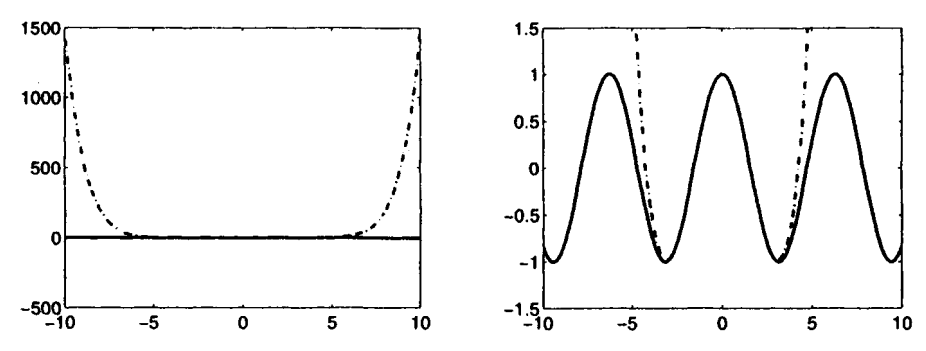
\includegraphics[max width=\textwidth]{fig22}
\caption{Graphs of $y=\cos (x)$ (solid) together with the eighth-order Taylor approximating polynomial $y=p_{8}(x)$ (dash-dot) shown with two different $y$-ranges.}
\label{fig:fig_2_2}
\end{figure}

To answer (even just) the first question, this plot is not going to help much, owing to the fact that the scale on the $y$-axis is so large (increments are in 200 units and we need our error to be $<0.2$). MATLAB always will choose the scales to accommodate all of the points in any given plot. The eighth-degree polynomial $y=p_{8}(x)$ gets so large at $x=\pm 10$ that the original function $y=\cos (x)$ is dwarfed in comparison so its graph will appear as a flat line (the $x$-axis). We could redo the plot trying out different ranges for the $x$-values and eventually arrive at a more satisfactory illustration.\footnote{ The zoom button \faSearchPluss \vspace{0.1cm}  on the graphics window can save some time here. To use it, simply left click on
this button with your mouse, then move the mouse to the desired center of the plot at which to zoom
and left click (repeatedly). The zoom-out key \faSearchMinuss \vspace{0.1cm}  works in the analogous fashion.} Alternatively and more simply, we can work with the existing plot and get MATLAB to manually change the range of the $x$ - and/or $y$-axes that appear in the plot. The way to do this is with the command:


$
\begin{array}{|l|l|}
\hline \begin{array}{l}
\text {axis([xmin xmax ymin ymax] } \rightarrow \\
\end{array} & \begin{array}{l}
\text {Changes the range of a plot to: } \\
\text {xmin $\leq$ x $\leq$ xmax  and ymin $\leq$ y $\leq$ ymax}\\

\end{array} \\
\hline
\end{array}
$\\

Thus to keep the $x$-range the same $[-10,10]$, but to change the $y$-range to be $[-1.5,1.5]$, we would enter the command to create the second plot of Figure 2.2.

\begin{verbatim}

>>axis([-1 0 10 -1. 5 1.5]) 

\end{verbatim}

We can see now from the second plot above that (certainly) for $-3 \leq x \leq 3$ we have $\left|\cos (x)-p_{8}(x)\right| \leq 0.2$. This graph is, however, unsatisfactory in regards to the second question of the determination of an $x$-interval for which $\left|\cos (x)-p_{8}(x)\right| \leq 0.001$. To answer this latter question and also to get a more satisfactory answer for the first question, we need only look at plots of the actual error $y=\left|\cos (x)-p_{8}(x)\right|$. We do this for two different $y$-ranges. There is a nice way to get MATLAB to partition its plot window into several (in fact, a matrix of) smaller subwindows.

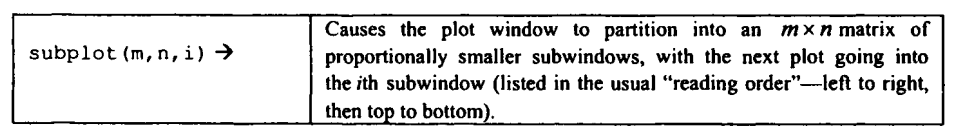
\includegraphics[max width=\textwidth]{tab17}

The two error plots in Figure $2.3$ were obtained with the following commands:

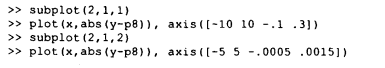
\includegraphics[max width=\textwidth]{code23}

Notice that the ranges for the axes were appropriately set for each plot so as to make each more suitable to answer each of the corresponding questions.

\begin{figure}[H]
\centering
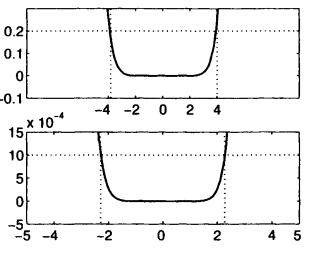
\includegraphics[max width=\textwidth]{fig23}
\caption{ Plots of the error $y=\left|\cos (x)-p_{8}(x)\right|$ on two different $y$-ranges. Reference lines were added to help answer the question in part (d) of Example $2.4$.}
\label{fig:fig_2_3}
\end{figure}

From Figure 2.3, we can deduce that if we want to guarantee an error of at most $0.2$, then we can use $p_{8}(x)$ to approximate $\cos (x)$ anywhere on the interval $[-3.8,3.8]$, while if we would like the maximum error to be only $0.001$, we must shrink the interval of approximation to about $[-2.2,2.2]$. In Figure $2.4$ we give a MATLAB-generated plot of the function $y=\cos (x)$ along with several of its Taylor polynomials.

\begin{figure}[H]
\centering
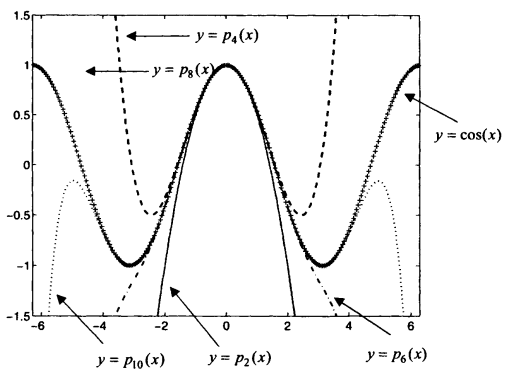
\includegraphics[max width=\textwidth]{fig24}
\caption{Some Taylor polynomials for $y=\cos (x)$.}
\label{fig:fig_2_4}
\end{figure}

EXERCISE FOR THE READER 2.1: Use MATLAB to produce the plot in Figure $2.4$ (without the arrow labels).

It is a rare situation indeed in numerical analysis where we can actually compute the exact errors explicitly. In the next section, we will give Taylor's theorem, which gives us usable estimates for the error even in cases where it cannot be explicitly computed.\\

\hrule width \hsize \kern 1pt \hrule width \hsize height 0.4pt

\hspace{0.1cm}

\textbf{EXERCISES 2.2: }

\begin{enumerate}
\item Find the second- and third-order Taylor polynomials $p_{2}(x)$ and $p_{3}(x)$, centered at $x=a$, for the each of the following functions.\\
(a) $f(x)=\sin (x), a=0$ \hspace{2.75cm} (b) $f(x)=\tan (x), a=0$\\
(c) $f(x)=e^{x}, a=1$ \hspace{3.50cm}(d) $f(x)=x^{1 / 3}, a=8$

\item Repeat Exercise 1 for each of the following:\\
(a) $f(x)=\cos (x), a=\pi / 2$\hspace{2.50cm} (b) $f(x)=\arctan (x), a=0$\\
(c) $f(x)=\ln x, a=1$ \hspace{3.25cm} (d) $f(x)=\cos \left(x^{2}\right), a=0$

\item (a) Approximate $\sqrt{65}$ by using the first-order Taylor polynomial of $f(x)=\sqrt{x}$ centered at $x=64$ (this is tangent line approximation discussed in first-semester calculus) and find the error and the relative error of this approximation.

(b) Repeat part (a) using instead the second-order Taylor polynomial to do the approximation.

(c) Repeat part (a) once again, now using the fourth-order Taylor polynomial.

\item (a) Approximate $\sin \left(92^{\circ}\right)$ by using the first-order Taylor polynomial of $f(x)=\sin (x)$ centered at $x=\pi / 2$ (tangent line approximation) and find the error and the relative error of this approximation

(b) Repeat part (a) using instead the second-order Taylor polynomial to do the approximation.

(c) Repeat part (a) using the fourth-order Taylor polynomial.

\item Find a general formula for the order $n$ Taylor polynomial $p_{n}(x)$ centered at $x=0$ for each of the following functions:\\

(a) $y=\sin (x)$ \hspace{3.75cm}(b) $y=\ln (1+x)$\\
(c) $y=e^{x}$\hspace{4.5cm}(d) $y=\sqrt{x+1}$

\item Find a general formula for the order $n$ Taylor polynomial $p_{n}(x)$ centered at $x=0$ for each of the following functions:\\
(a) $y=\tan (x)$ \hspace{3.75cm}(b) $y=1 /(1+x)$\\
(c) $y=\arctan (x)$ \hspace{3.30cm}(d) $y=x \sin (x)$

\item (a) Compute the following Taylor polynomials, centered at $x=0$, of $y=\cos \left(x^{2}\right)$ :

$$
p_{1}(x), p_{2}(x), p_{6}(x), p_{10}(x)
$$

(b) Next, use the general formula obtained in Example $2.4$ for the general Taylor polynomials of $y=\cos (x)$ to write down the order $0,1,3$, and 5 Taylor polynomials. Replace $x$ with $x^{2}$ in each of these polynomials. Compare these with the Taylor polynomials in part (a). 

\item Consider the function $f(x)=\sin (3 x)$. All of the plots in this problem are to be done with MATLAB on the interval $[-3,3]$. The Taylor polynomials refer to those of $f(x)$ centered at $x=0$. Each graph of $f(x)$ should be done with the usual plot settings, while each graph of a Taylor polynomial should be done with the dot style.

$
\begin{array}{|l|l|}
\hline \begin{array}{l}
\text {The simultaneous graphs of $f(x)$ along with}\\
\text {the 1st-order Taylor polynomial (= tangent line)}
\end{array} & \begin{array}{l}
\text { A graph of the error $\left|f(x)-p_{1}(x)\right|$}
\end{array} \\
\hline \begin{array}{l}
\text {The simultaneous graphs of $f(x)$ along with}\\
\text {the 3rd-order Taylor polynomial}
\end{array} & \begin{array}{l}
\text { A graph of the error $\left|f(x)-p_{3}(x)\right|$}
\end{array} \\
\hline \begin{array}{l}
\text {The simultaneous graphs of $f(x)$ along with)}\\
\text {the 9rd-order Taylor polynomial}
\end{array} & \begin{array}{l}
\text { A graph of the error $\left|f(x)-p_{9}(x)\right|$}
\end{array} \\
\hline
\end{array}
$ \\



\item (a) Let $f(x)=\ln \left(1+x^{2}\right)$. Find formulas for the following Taylor polynomials of $f(x)$ centered at $x=0: p_{2}(x), p_{3}(x), p_{6}(x)$. Next, using the subplot command, create a graphic window split in two sides (left and right). On the left, plot (together) the four functions $f(x)$, $p_{2}(x), p_{3}(x), p_{6}(x)$. In the right-side subwindow, plot (together) the corresponding graphs of the three errors: $\left|f(x)-p_{2}(x)\right|,\left|f(x)-p_{3}(x)\right|$, and $\left|f(x)-p_{6}(x)\right|$. For the error plot adjust the $y$-range so as to make it simple to answer the question in part (b). Use different styles/colors to code different functions in a given plot.

\item(a) Let $f(x)=x^{2} \sin (x)$. Find formulas for the following Taylor polynomials of $f(x)$ centered at $x=0: p_{1}(x), p_{4}(x), p_{9}(x)$. Next, using the subplot command, get MATLAB to create a graphic window split in two sides (left, and right). On the left, plot (together) the four functions $f(x), p_{1}(x), p_{4}(x), p_{9}(x)$. In the right-side subwindow, plot (together) the corresponding graphs of the three errors: $\left|f(x)-p_{1}(x)\right|,\left|f(x)-p_{4}(x)\right|$, and $\left|f(x)-p_{9}(x)\right|$. For the error plot adjust the $y$-range so as to make it simple to answer the question in part (b). Use different styles/colors to code different functions in a given plot.

\item In Example 2.3, we derived the general formula (2) for the zero- and first-order Taylor polynomial.

(a) Do the same for the second-order Taylor polynomial, i.e., use the definition of the Taylor polynomial $p_{2}(x)$ to show that $(2)$ is valid when $n=2$.

(b) Prove that formula (4) for the Taylor polynomials centered at $x=0$ is valid for any $n$.

(c) Prove that formula (2) is valid for all $n$.

\textbf{Suggestion:} For part (c), consider the function $g(x)=f(x+a)$, and apply the result of part (b) to this function. How are the Taylor polynomials of $g(x)$ at $x=0$ related to those of $f(x)$ at $x=a$ ?

\item \emph{(Another Kind of Polynomial Interpolation)} In this problem we compare the fourth-order Taylor polynomial $p_{3}(x)$ of $y=\cos (x)$ at $x=0$ (which is actually $p_{4}(x)$ ) with the third-order polynomial $p(x)=a_{0}+a_{1} x+a_{2}^{\prime} x^{2}+a_{3} x^{3}$, which has the same values and derivative as $\cos (x)$ at the points $x=0$ and $x=\pi$. This means that $p(x)$ satisfies these four conditions:

$$
p(0)=1 \quad p^{\prime}(0)=0 \quad p(\pi)=-1 \quad p^{\prime}(\pi)=0
$$
Find the coefficients: $a_{0}, a_{1}, a_{2}$, and $a_{3}$ of $p(x)$, and then plot all three functions together. Discuss the errors of the two different approximating polynomials.
\end{enumerate}

\section{TAYLOR'S THEOREM}

\begin{wrapfigure}{l}{0.25\textwidth}
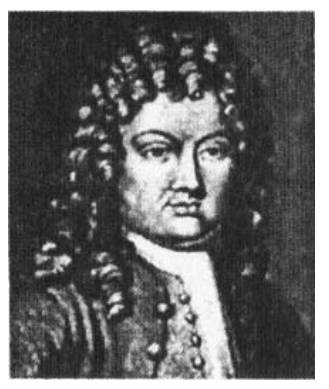
\includegraphics[width=0.9\linewidth]{fig25} 
\caption{Brook Taylor (1685-1731), English mathematician \protect\footnotemark[2]}
\label{fig:fig_2_5}
\end{wrapfigure}

In the examples and problems of previous section we introduced Taylor polynomials $p_{n}(x)$ of a function $y=f(x)$
(appropriately differentiable) at $x=a$, and we saw that they appear to often serve as great tools for approximating the function near $x=a$. We also have seen that as the order $n$ of the Taylor polynomial increases, so does its effectiveness in approximating $f(x)$. This of course needs to be reconciled with the fact that for larger values of $n$ it is more work to form and compute $p_{n}(x)$. Additionally, the approximations seemed to improve, in general, when $x$ gets closer to $a$. This latter observation seems plausible since $p_{n}(x)$ was  constructed using only information about $f(x)$ at provides precise quantitative estimates for the error $x=a$. Taylor's theorem provides precise quantitative estimates for the error $\left|f(x)-p_{n}(x)\right|$, which can be very useful in choosing an appropriate order $n$ so that $p_{n}(x)$ will give an approximation within the desired error bounds. We now present Taylor's theorem. For its proof we refer the reader to any decent calculus textbook.\\


\footnotetext[2]{Taylor was born in Middlesex, England, and his parents were quite well-rounded people of society.
His father was rather strict but instilled in Taylor a love for music and painting. His parents had him
educated at home by private tutors until he entered St. John's College in Cambridge when he was 18.
He graduated in 1709 after having written his first important mathematical paper a year earlier (this
paper was published in 1714). He was elected rather early in his life (1712) to the Royal Society, the
election being based more on his potential and perceived mathematical powers rather than on his
published works, and two years later he was appointed to the prestigious post of Secretary of the Royal
Society. In this same year he was appointed to an important committee that was to settle the issue of
"who invented calculus" since both Newton and Leibniz claimed to be the founders. Between 1712
and 1724 Taylor published 13 important mathematical papers on a wide range of subjects including
magnetism, logarithms, and capillary action.
Taylor suffered some tragic personal events. His father objected to his marriage (claiming the bride's
family was not a "good" one) and after the marriage Taylor and his father cut off all contact until 1723,
when his wife died giving birth to what would have been Taylor's first child. Two years later he
remarried (this time with his father's blessings) but the following year his new wife also died during
childbirth, although this time his daughter survived. }

\noindent \textbf{THEOREM 2.1:} \emph{(Taylor's Theorem)} Suppose that for a positive integer $n$, a function $f(x)$ has the property that its $(n+1)$ st derivative is continuous on some interval $I$ on the $x$-axis that contains the value $x=a$. Then the $n$ th-order remainder $R_{n}(x) \equiv f(x)-p_{n}(x)$ resulting from approximating $f(x)$ by $p_{n}(x)$ is given by

\begin{equation} \label{eq:5} \tag{5}
R_{n}(x)=\frac{f^{(n+1)}(c)}{(n+1) !}(x-a)^{n+1} \quad(x \in I),
\end{equation}

for some number $c$, lying between $a$ and $x$ (inclusive); see Figure 2.6.


\begin{figure}[H]
\centering
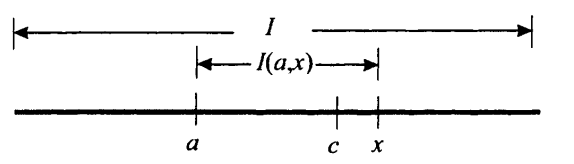
\includegraphics[max width=\textwidth]{fig26}
\caption{One possible arrangement of the three points relevant to Taylor's theorem.}
\label{fig:fig_2_6}
\end{figure}

REMARKS: (1) Note that like many such theorems in calculus, Taylor's theorem asserts the existence of the number $c$, but it does not tell us what it is.

(2) By its definition, (the absolute value of) $R_{n}(x)$ is just the actual error of the approximation of $f(x)$ by its $n$ th-order Taylor polynomial $p_{n}(x)$, i.e.,
$$
\text { error }=\left|f(x)-p_{n}(x)\right|=\left|R_{n}(x)\right| .
$$
Since we do not know the exact value of $c$, we will not be able to calculate the error precisely; however, since we know that $c$ must lie somewhere between $a$ and $x$ on $I$, call this interval $I(a, x)$, we can estimate that the unknown quantity $\left|f^{(n+1)}(c)\right|$ that appears in $R_{n}(x)$, can be no more than the maximum value of this $(n+1)$ st derivative function $\left|f^{(n+1)}(z)\right|$ as $z$ runs through the interval $I(a, x)$. In mathematical symbols, this is expressed as:

\begin{equation} \label{eq:6} \tag{6}
\left|f^{(n+1)}(c)\right| \leq \max \left\{\left|f^{(n+1)}(z)\right|: z \in I(a, x)\right\} .
\end{equation}


\textbf{EXAMPLE 2.5:} Suppose that we wish to use Taylor polynomials (at $x=0$ ) to approximate $e^{0.7}$ with an error less than $0.0001$. 

(a) Apply Taylor's theorem to find out what order $n$ of a Taylor polynomial we could use for the approximation to guarantee the desired accuracy.

(b) Perform this approximation and then check that the actual error is less than maximum tolerated error.\\

SOLUTION: Part (a): Here $f(x)=e^{x}$, so, since $f(x)$ is its own derivative, we have $f^{(n)}(x)=e^{x}$ for any $n$, and so $f^{(n)}(0)=e^{0}=1$. From (4) (or (2) or (3) with $a=0)$, we can therefore write the general Taylor polynomial for $f(x)$ centered at $x=0$ as
$$
p_{n}(x)=1+x+\frac{x^{2}}{2 !}+\frac{x^{3}}{3 !}+\cdots+\frac{x^{n}}{n !}=\sum_{k=0}^{n} \frac{x^{k}}{k !},
$$
and from (5) (again with $a=0), R_{n}(0.7)=\frac{e^{c}}{(n+1) !}(0.7)^{n+1}$.

How big can $e^{c}$ be? For $f(x)=e^{x}$, this is just the question of finding out the right side of (6). In this case the answer is easy: Since $c$ lies between 0 and 0.7, and $e^{x}$ is an increasing function, the largest value that $e^{c}$ can be is $e^{0.7}$. To honestly use Taylor's theorem here (since "we do not know" what $e^{0.7}$ is-that's what we are trying to approximate), let's use the conservative upper bound: $e^{c} \leq e^{0.7} \leq e^{1}=e<3$.

Now Taylor's theorem tells us that
$$
\text { error }=\left|e^{0.7}-p_{n}(0.7)\right|=\left|R_{n}(0.7)\right|=\frac{e^{c}}{(n+1) !}(0.7)^{n+1} .
$$
(Since all numbers on the right side are nonnegative, we are able to drop absolute value signs.) As was seen above, we can replace $e^{c}$ with 3 in the right side above, to get
$$
\text { something larger than the error }=\frac{3}{(n+1) !}(0.7)^{n+1} \text {. }
$$

The rest of the plan is simple: We find an $n$ large enough to make the "something larger than actual error" to be less than the desired accuracy $0.0001$. Then it will certainly follow that the actual error will also be less than $0.0001$. We can continue to compute $3(0.7)^{n+1} /(n+1)$ ! until it gets smaller than $0.0001$. Better yet, let's use a while loop to get MATLAB to do the work for us; this will also provide us with a good occasion to introduce the remaining relational operators that can be used in any while loops (or subsequent programming). (See Table 2.1.)

$
\begin{aligned}
\centering
&\text { Table 2.1: Dictionary of MATLAB's relational operators. }\\
&\begin{array}{|c|c|}
\hline \text { Mathematical Relation } & \text { MATLAB Code } \\
\hline>,< & >,< \\
\hline \geq, \leq & >=, \quad<= \\
\hline=\neq & ==, \quad \sim= \\
\hline
\end{array}
\end{aligned}
$

We have already used one of the first pair. For the last one, we reiterate again that the single equal sign in MATLAB is reserved for "assignment." Since it gets used much less often (in MATLAB codes), the ordinary equals in mathematics got stuck with the more cumbersome MATLAB notation.

Now, back to our problem. A simple way to figure out that smallest feasible value of $n$ would be to run the following code:


\begin{verbatim}
>> n=1;
>>while 3*(0.7)^(n+1)/gamma(n+2) >= 0.0001
	n=n+1;
end
\end{verbatim}

This code has no output, but what it does is to keep making $n$ bigger, one-by-one, until that "something larger than the actual error" gets less than $0.0001$. The magic value of $n$ that will work is now (by the way the while loop was constructed) simply the last stored value of $n$ :

$>>n \rightarrow 6$

Part (b): The desired approximation is now: $e^{0.7} \approx p_{6}(0.7)=\left.\sum_{k=0}^{6} \frac{(0.7)^{k}}{k !}\right|_{x=0.7}$.

We can do the rest on MATLAB:

\begin{verbatim}
>>x=0.7;
>> n=0;
>>p6=0; % we initialize the sum for the Taylor polynomial p6
>>while n<=6;
	p6-p6+x^n/gamma(n+1); 
	n=n+1;
end
>>p6
->2.0137 (approximation)
>> abs(p6-exp (0.7)) %we now check the actual error
->» 1.7889e-005 (this is less than 0.0001, as we knew from Taylor's theorem.)
\end{verbatim}

EXERCISE FOR THE READER 2.2: If we use Taylor polynomials of $f(x)=\sqrt{x}$ centered at $x=16$ to approximate $\sqrt{17}=f(16+1)$, what order Taylor polynomial should be used to ensure that the error of the approximation is less than $10^{-10}$ ? Perform this approximation and then look at the actual error. For any function $f(x)$, which has infinitely many derivatives at $x=a$, we can form the \textbf{Taylor series (centered) at} $x=a$ :
$$
\begin{aligned}
&f(a)+f^{\prime}(a)(x-a)+\frac{f^{\prime \prime}(a)}{2}(x-a)^{2}+\frac{f^{\prime \prime \prime}(a)}{3 !}(x-a)^{3}+\cdots \\
&+\frac{f^{(n)}(a)}{n !}(x-a)^{n}+\cdots=\sum_{k=0}^{\infty} \frac{f^{(k)}(a)}{k !}(x-a)^{k} .
\end{aligned}
$$

Comparing this with (2) and (3), the formulas for the $n$th Taylor polynomial $p_{n}(x)$ at $x=a$, we see that the Taylor series is just the infinite series whose first $n$ terms are exactly the same as those of $p_{n}(x)$. The Taylor series may or may not converge, but if Taylor's theorem shows that the errors $\left|p_{n}(x)-f(x)\right|$ go to zero, then it will follow that the Taylor series above converges to $f(x)$. When $a=0$ (the most common situation), the series is called the Maclaurin series (Figure 2.7).

It is useful to have some Maclaurin series for reference. Anytime we are able to figure out a formula for the general Taylor polynomial at $x=0$, we can write down the corresponding Maclaurin series. The previous examples we have done yield the Maclaurin series for $\cos (x)$ and $e^{x}$. We list these in Table 2.2, as well as a few other examples whose derivations will be left to the exercises.

$
\begin{aligned}
\centering
&\text { Table 2.1: Some Maclaurin series expansions. }\\
&\begin{array}{|l|l|l|}
\hline \text { Function Nactaurin Series } & \text {Maclaurian Series } \\
\hline e^{x} & 1+x+\frac{x^{2}}{2 !}+\frac{x^{3}}{3 !}+\cdots+\frac{x^{k}}{k !}+\cdots \label{eq:8} & (8) \\
\hline \cos (x) & 1-\frac{x^{2}}{2 !}+\frac{x^{4}}{4 !}+\cdots+\frac{(-1)^{k} x^{2 k}}{(2 k) !}+\cdots \label{eq:9} & (9) \\
\hline \sin (x) & x-\frac{x^{3}}{3 !}+\frac{x^{5}}{5 !} \cdots+\frac{(-1)^{k} x^{2 k+1}}{(2 k+1) !}+\cdots  \label{eq:10} & (10) \\
\hline \arctan (x) & x-\frac{x^{3}}{3}+\frac{x^{5}}{5}-\cdots+\frac{(-1)^{2 k+1} x^{2 k+1}}{2 k+1}+\cdots  \label{eq:11} & (11) \\
\hline \frac{1}{1-x} & 1+x+x^{2}+x^{3}+\cdots+x^{k}+\cdots  \label{eq:12} &(12) \\
\hline
\end{array}
\end{aligned}
$\\

One very useful aspect of Maclaurin and Taylor series is that they can be formally combined to obtain new Maclaurin series by all of the algebraic operations (addition, subtraction, multiplication, and division) as well as with substitutions, derivatives, and integrations. These informally obtained expansions are proved to be legitimate in calculus books. The word "formal" here means that all of the above operations on an infinite series should be done as if it were a finite sum. This method is illustrated in the next example.

\begin{wrapfigure}{l}{0.35\textwidth}

\includegraphics[width=0.9\linewidth]{fig27} 
\caption{Brook Taylor (1685-1731), English mathematician \protect\footnotemark[3]}
\label{fig:fig_2_7}
\end{wrapfigure}

\textbf{EXAMPLE 2.6}: Using formal manipulations, obtain the Maclaurin series of the functions (a) $x \sin \left(x^{2}\right)$ and $(b) \ln \left(1+x^{2}\right)$.
 
SOLUTION: Part (a): In (10) simply replace $x$ with $x^{2}$ and formally multiply by $x$ (we use the symbol $\sim$ to mean "has the Maclaurin series"):
$$
\begin{aligned}
&x \sin \left(x^{2}\right) \sim \\
&x\left(x^{2}-\frac{\left(x^{2}\right)^{3}}{3 !}+\frac{\left(x^{2}\right)^{5}}{5 !} \cdots+\frac{(-1)^{k}\left(x^{2}\right)^{2 k+1}}{(2 k+1) !}\right. \\
&=x^{3}-\frac{x^{7}}{3 !}+\frac{x^{11}}{5 !} \cdots+\frac{(-1)^{k} x^{4 k+3}}{(2 k+1) !}+\cdots
\end{aligned}
$$

\noindent NOTE: This would have been a lot more work to do by using the definition and looking for patterns.

Part (b): We first formally integrate (12): $-\ln (1-x)$
$$
\sim \int\left(1+x+x^{2}+x^{3}+\cdots+x^{n}+\cdots\right) d x=C+x+\frac{x^{2}}{2}+\frac{x^{3}}{3}+\cdots+\frac{x^{n+1}}{n+1}+\cdots .
$$

By making $x=0$, we get that the integration constant $C$ equals zero. Now negate both sides and substitute $x$ with $-x^{2}$ to obtain:

$$
\begin{aligned}
\ln \left(1+x^{2}\right) & \sim x^{2}-\frac{\left(-x^{2}\right)^{2}}{2}-\frac{\left(-x^{2}\right)^{3}}{3}-\cdots-\frac{\left(-x^{2}\right)^{n+1}}{n+1}-\cdots \\
& \sim x^{2}-\frac{x^{4}}{2}+\frac{x^{6}}{3}-\cdots+\frac{(-1)^{k+1} x^{2 k}}{k}+\cdots
\end{aligned}
$$


\footnotetext[3]{Maclaurin was born in a small village on the river Ruel in Scotland. His father, who was the village 
minister, died when Colin was only six weeks old. His mother wanted Colin and his brother John to 
have good education so she moved the family to Dumbarton, which had reputable schools. Col in's 
mother died when he was only nine years old and he subsequently was cared for by his uncle, also a 
minister. Colin began studies at Glasgow University when he was 11 years old (it was more common 
during these times in Scotland for bright youngsters to begin their university studies early—in fact 
universities competed for them). He graduated at age 14 when he defended an impressive thesis 
extending Sir Isaak Newton's theory on gravity. He then went on to divinity school with the intention 
of becoming a minister, but he soon ended this career path and became a chaired mathematics professor 
at the University of Aberdeen in 1717 at age 19. 
Two years later, Maclaurin met the illustrious Sir Isaak Newton and they became good friends. The 
latter was instrumental in Maclaurin's appointment in this same year as a Fellow of the Royal Society 
(the highest honor awarded to English academicians) and subsequently in 1725 being appointed to the 
faculty of the prestigious University of Edinburgh, where he remained for the rest of his career. 
Maclaurin wrote several important mathematical works, one of which was a joint work with the very 
famous Leonhard Euler and Daniel Bernoulli on the theory of tides, which was published in 1740 and 
won the three a coveted prize from the Académie des Sciences in Paris. Maclaurin was also known as 
an excellent and caring teacher. He married in 1733 and had seven children. He was also known for 
his kindness and had many friends, including members of the royalty. He was instrumental in his work 
at the Royal Society of Edinburgh, having it transformed from a purely medical society to a more 
comprehensive scientific society. During the 1745 invasion of the Jacobite army, Maclaurin was 
engaged in hard physical labor in the defense of Edinburgh. This work, coupled with an injury from 
falling off his horse, weakened him to such an extent that he died the following year. }

Our next example involves another approximation using Taylor's theorem. Unlike the preceding approximation examples, this one involves an integral where it is impossible to find the antiderivative.

\textbf{EXAMPLE 2.7:} Use Taylor's theorem to evaluate the integral $\int_{0}^{1} \sin \left(t^{2}\right) d t$ with an error $<10^{-7}$.

SOLUTION: Let us denote the $n$ th-order Taylor polynomial of $\sin (x)$ centered at $x=0$ by $p_{n}(x)$. The formulas for each $p_{n}(x)$ are easily obtained from the Maclaurin series (10). We will estimate $\int_{0}^{1} \sin \left(t^{2}\right) d t$ by $\int_{0}^{1} p_{n}\left(t^{2}\right) d t$ for an appropriately large $n$. We can easily obtain an upper bound for the error of this approximation:
$$
\text { error }=\left|\int_{0}^{1} \sin \left(t^{2}\right) d t-\int_{0}^{1} p_{n}\left(t^{2}\right) d t\right| \leq \int_{0}^{1}\left|\sin \left(t^{2}\right)-p_{n}\left(t^{2}\right)\right| d t \leq \int_{0}^{1}\left|R_{n}\left(t^{2}\right)\right| d t \text {, }
$$
where $R_{n}(x)$ denotes Taylor's remainder. Since any derivative of $f(x)=\sin (x)$ is one of $\pm \sin (x)$ or $\pm \cos (x)$, it follows that for any $x, 0 \leq x \leq 1$, we have
$$
\left|R_{n}(x)\right|=\left|\frac{f^{(n+1)}(c) x^{n+1}}{(n+1) !}\right| \leq \frac{1}{(n+1) !} .
$$
Since in the above integrals, $t$ is running from $t=0$ to $t=1$, we can substitute $x=t^{2}$ in this estimate for $\left|R_{n}(x)\right|$. We can use this and continue with the error estimate for the integral to arrive at:
$$
\text { error }=\left|\int_{0}^{1} \sin \left(t^{2}\right) d t-\int_{0}^{1} p_{n}\left(t^{2}\right) d t\right| \leq \int_{0}^{1}\left|R_{n}\left(t^{2}\right)\right| d t \leq \int_{0}^{1} \frac{d t}{(n+1) !}=\frac{1}{(n+1) !} .
$$
As in the previous example, let's now get MATLAB to do the rest of the work for us. We first need to determine how large $n$ must be so that the right side above (and hence the actual error) will be less than $10^{-7}$.

\begin{verbatim}
>>n = 1;
>>while 1/gamma(n+2) >= 10^(-7)
	n=n+1;
end
>>n -> 10
\end{verbatim}

So it will be enough to replace $\sin \left(t^{2}\right) 10$ th-order Taylor polynomial evaluated at $t^{2}, p_{n}\left(t^{2}\right)$. The simplest way to see the general form of this polynomial (and its integral) will be to replace $x$ with $t^{2}$ in the Maclaurin series (10) and then formally integrate it (this will result in the Maclaurin series for $\int_{0}^{x} \sin \left(t^{2}\right) d t$ ):

If we substitute $x=0$, we see that the constant of integration $C$ equals zero. Thus,
$$
\int_{0}^{x} \sin \left(t^{2}\right) d t \sim \frac{x^{3}}{3}-\frac{x^{7}}{7 \cdot 3 !}+\frac{x^{11}}{11 \cdot 5 !}+\cdots+\frac{(-1)^{k} x^{4 k+3}}{(4 k+3) \cdot(2 k+1) !}+\cdots .
$$
We point out that the formal manipulation here is not really necessary since we could have obtained from (10) an explicit formula for $p_{10}\left(t^{2}\right)$ and then directly integrated this function. In either case, integrating this function from $t=0$ to $t=1$ gives the partial sum of the last Maclaurin expansion (for $\int_{0}^{x} \sin \left(t^{2}\right) d t$ ) gotten by going up to the $k=4$ term, since this corresponds to integrating up through the terms of $p_{10}\left(t^{2}\right)$.

\begin{verbatim}
>>p10=0 ;
>>k=0;
>>while k<=4
	p10=p10+(-1)^k/(4*k+3)/gamma(2*k+2) ;
	k = k+1;
end
>>format long
>> p10S
->p10 = 0.31026830280668
\end{verbatim}

In summary, we have proved the approximation
$$
\int_{0}^{1} \sin \left(t^{2}\right) d t \approx 0.31026830280668 .
$$
Taylor's theorem has guaranteed that this is accurate with an error less than $10^{-7}$.\\

EXERCISE FOR THE READER 2.3: Using formal manipulations, find the 10thorder Taylor polynomial centered at $x=0$ for each of the following functions: (a) $\sin \left(x^{2}\right)-\cos \left(x^{3}\right)$, (b) $\sin ^{2}\left(x^{2}\right)$.
$$
\begin{aligned}
& \sin \left(t^{2}\right) \sim t^{2}-\frac{t^{6}}{3 !}+\frac{t^{10}}{5 !} \cdots+\frac{(-1)^{k} t^{4 k+2}}{(2 k+1) !}+\cdots \Rightarrow \\
& \int_{0}^{x} \sin \left(t^{2}\right) d t \sim \int_{0}^{x}\left(t^{2}-\frac{t^{6}}{3 !}+\frac{t^{10}}{5 !}+\cdots+\frac{(-1)^{k} t^{4 k+2}}{(2 k+1) !}+\cdots\right) d t \\
& \sim C+\frac{x^{3}}{3}-\frac{x^{7}}{7 \cdot 3 !}+\frac{x^{11}}{11 \cdot 5 !}+\cdots+\frac{(-1)^{k} x^{4 k+3}}{(4 k+3) \cdot(2 k+1) !}+\cdots . 
\end{aligned}
$$

\hrule width \hsize \kern 1pt \hrule width \hsize height 0.4pt

\hspace{0.1cm}

\textbf{EXERCISES 2.3: }

\begin{enumerate}
\item In each part below, we give a function $f(x)$, a center a to use for Taylor polynomials, a value for $x$, and a positive number $\varepsilon$ that will stand for the error. The task will be to (carefully) use Taylor's theorem to find a value of the order $n$ of a Taylor polynomial so that the error of the approximation $f(x) \approx p_{n}(x)$ is less than $\varepsilon$. Afterward, perform this approximation and check that the actual error is really less than what it was desired to be.\\
(a) $f(x)=\sin (x), a=0, x=0.2 \mathrm{rad}, \varepsilon=0.0001$\\
(b) $f(x)=\tan (x), a=0, x=5^{\circ}, \varepsilon=0.0001$\\
(c) $f(x)=e^{x}, a=0, x=-0.4, \varepsilon=0.00001$\\
(d) $f(x)=x^{1 / 3}, a=27, x=28, \varepsilon=10^{-6}$

\item Follow the directions in Exercise 1 for the following:\\
(a) $f(x)=\cos (x), a=\pi / 2, x=88^{\circ}, \varepsilon=0.0001$\\
(b) $f(x)=\arctan (x), a=0, x=1 / 239, \varepsilon=10^{-8}$\\
(c) $f(x)=\ln x, a=1, x=3, \varepsilon=0.00001$\\
(d) $f(x)=\cos \left(x^{2}\right), a=0, x=2.2, \varepsilon=10^{-6}$

\item Using only the Maclaurin series developed in this section, along with formal manipulations, obtain Maclaurin series for the following functions:\\
(a) $x^{2} \arctan (x)$\\
(b) $\ln (1+x)$\\
(c) $\frac{x^{2}+3 x}{1-x}$\\
(d) $\int_{0}^{x} \frac{1}{1-t^{3}} d t$

\item Using only the Maclaurin series developed in this section, along with formal manipulations, obtain Maclaurin series for the following functions:\\
(a) $\ln (1+x)$\\
(b) $1 /\left(1+x^{2}\right)$\\
(c) $\arctan \left(x^{2}\right)-\sin (x)$\\
(d) $\int_{0}^{x} \cos \left(t^{5}\right) d t$

\item Find the Maclaurin series for $f(x)=\sqrt{1+x}$.

\item Find the Maclaurin series for $f(x)=(1+x)^{1 / 3}$.

\item (a) Use Taylor's theorem to approximate the integral $\int_{0}^{1} \cos \left(t^{5}\right) d t$ with an error less than $10^{-8}$. (First find a large enough order $n$ for a Taylor polynomial that can be used from the theorem, then actually perform the approximation.)\\
(b) How large would $n$ have to be if we wanted the error to be less than $10^{-30}$ ?

\item The error function is given by the formula: erf $(x)=(2 / \sqrt{\pi}) \int_{0}^{x} e^{-t^{2}} d t$. It is used extensively in probability theory, but unfortunately the integral cannot be evaluated exactly. Use Taylor's theorem to approximate erf( 2$)$ with an error less than $10^{-6}$.

\item Since $\tan (\pi / 4)=1$ we obtain $\pi=4 \arctan (1)$. Using the Taylor series for the arctangent, this gives us a scheme to approximate $\pi$.

(a) Using Taylor polynomials of $\arctan (x)$ centered at $x=0$, how large an order $n$ Taylor polynomial would we need to use in order for $4 p_{n}(1)$ to approximate $\pi$ with an error less than $10^{-12} ?$

(b) Perform this approximation.

(c) How large an order $n$ would we need for Taylor's theorem to guarantee that $4 p_{n}(1)$ approximates $\pi$ with an error less than $10^{-50} ?\footnote[4]{Of course, since MATLAB's compiler keeps track of only about 15 digits, such an accurate 
approximation could not be done without the help of the Symbolic Toolbox (see Appendix A).}$

(d) There are more efficient ways to compute $\pi$. One of these dates back to the early 1700 s, when Scottish mathematician John Machin (1680-1751) developed the inverse trig identity:
\begin{equation}\label{eq:13} \tag{13}
\frac{\pi}{4}=\arctan \left(\frac{1}{5}\right)-\arctan \left(\frac{1}{239}\right)
\end{equation}
to calculate the first 100 decimal places of $\pi$. There were no computers back then, so his work was all done by hand and it was important to do it in way where not so many terms needed to be computed. He did it by using Taylor polynomials to approximate each of the two arctangents on the right side of (13). What order Taylor polynomials would Machin have needed to use (according to Taylor's theorem) to attain his desired accuracy?

(e) Prove identity (13).

Suggestion: For part (d), use the trig identity:
$$
\tan (A \pm B)=\frac{\tan A \pm \tan B}{1 \mp \tan A \tan B}
$$
to calculate first $\tan \left(2 \tan ^{-1} \frac{1}{5}\right)$, then $\tan \left(4 \tan ^{-1} \frac{1}{5}\right)$, and finally $\tan \left(4 \tan ^{-1} \frac{1}{5}-\tan ^{-1} \frac{1}{239}\right)$.\\

HISTORICAL ASIDE: Since antiquity, the problem of figuring out $\pi$ to more and more decimals has challenged the mathematical world, and in more recent times the computer world as well. Such tasks can test the powers of computers as well as the methods used to compute them. Even in the 1970 s $\pi$ had been calculated to over 1 million places, and this breakthrough was accomplished using an identity quite similar to (13). See [Bec-71] for an enlightening account of this very interesting history.

\item \emph{(Numerical Differentiation)} (a) Use Taylor's theorem to establish the following \emph{forward difference formula}:

$$
f^{\prime}(a)=\frac{f(a+h)-f(a)}{h}-\frac{h}{2} f^{\prime \prime}(c),
$$

for some number $c$ between $a$ and $a+h$, provided that $f^{\prime}(x)$ is continuous on $[a, a+h]$. This formula is often used as a means of numerically approximating the derivative $f^{\prime}(a)$ by the simple difference quotient on the right; in this case the error of the approximation would be $\left|h f^{\prime \prime}(c) / 2\right|$ and could be made arbitrarily small if we take $h$ sufficiently small.

(b) With $f(x)=\sinh (x)$, and $a=0$, how small would we need to take $h$ for the approximation in part (a) to have error less than $10^{-5}$ ? Do this by first estimating the error, and then (using your value of $h$ ) check the actual error using MATLAB. Repeat with an error goal of $10^{-10}$.

(c) Use Taylor's theorem to establish the following central difference formula:
$$
f^{\prime \prime}(a)=\frac{f(a+h)-2 f(a)+f(a+h)}{h^{2}}-\frac{h^{2}}{12} f^{(4)}(c)
$$
for some number $c$ between $a-h$ and $a+h$, provided that $f^{(4)}(x)$ is continuous on $[a-h, a+h]$. This formula is often used as a means of numerically approximating the derivative $f^{\prime \prime}(a)$ by the simple difference quotient on the right; in this case the error of the approximation would be $\left|h^{2} f^{(4)}(c) / 12\right|$ and could be made arbitrarily small if we take $h$ sufficiently small.

(d) Repeat part (b) for the approximation of part (c). Why do the approximations of part (c) seem more efficient, in that they do not require as small an $h$ to achieve the same accuracy?

(e) Can you derive (and prove using Taylor's theorem) an approximation for $f^{\prime}(x)$ whose error is proportional to $h^{2}$ ?

\end{enumerate}

\end{document}